\chapter{基于4PCS的位姿估计算法}
\label{chap:matcher}
本章主要介绍一种基于4PCS的位姿估计算法4PCS-PE(4PCS-based Pose Estimation),4PCS-PE主要基于全局匹配算法4PCS\cite{aiger20084}和局部匹配算法ICP\cite{besl1992method}。为了详细介绍4PCS-PE算法,本章首先从整体上简单介绍了4PCS-PE算法,包括算法所要解决的问题的具体数学描述以及相关算法的背景;然后介绍4PCS-PE算法的基础4PCS算法,并分析了其不足,进而引入改进的4PCS算法;接着介绍与改进的4PCS算法相结合的ICP算法,ICP算法主要用于提高最终位姿估计的精度;最后进行了位姿估计的实验,将本文的4PCS-PE算法与其他几个位姿估计算法相比较。

\section{位姿估计算法概述}
\subsection{问题描述}
通过第~\ref{chap:detector}~章中的目标检测算法可以得到目标的bounding box或者mask,根据bounding box或者mask可以在深度图中提取对应的区域,从而获得包含目标的点云。所以现在的问题是如何通过目标的点云计算出目标的位姿,由于可以得到目标的三维模型,因此将目标的三维模型经过一个刚体变换$T$,使之与目标点云重合,然后目标的三维模型在相机坐标系下的位姿也是已知并且可调的,为方便起见将三维模型坐标系与相机坐标系重合,则目标的位姿便等于三维模型与目标点云之间的齐次变换关系,即$T$。所以,要计算目标的位姿,就要求解目标三维模型与相机采集到的目标点云之间的刚体变换$T$,如图~\ref{fig:match_diagram}~,这也是4PCS-PE主要要解决的问题。
\begin{figure}[ht]
  \centering
  \includegraphics[width=14cm]{match_diagram}
  \caption{位姿估计示意图}
  \label{fig:match_diagram}
\end{figure}

相机所采集到的目标点云是一组包含空间三维坐标(x,y,z)以及颜色(r,g,b)的点集\footnote{对点集(point set)与点云(point cloud)不做区分,都指包含坐标点的集合},由于此处并不需要颜色信息,因此对目标点云只保留空间位置信息,去除颜色信息后的目标点云记为点集$P$。三维模型亦可通过采样得到一组包含空间三维坐标的点集,记为$Q$。4PCS-PE算法就可以简化为求解一个刚体变换$T$使得点集$P$中的点经过矩阵$T$变换后,尽可能与点集$Q$重合。更为准确地,4PCS-PE算法就可以简化为求解一个LCP(Largest Common Pointset)问题:

{\kai LCP问题:给定两个点集$P$和$Q$,在给定距离误差$\delta$下,求解点集$P$的最大子集$P'$,使得$T(P')$和点集$Q$之间的距离在合适的距离度量下小于$\delta$,其中$T$是一个刚体变换。}

\subsection{背景介绍}
LCP问题并不是一个新的问题,解决该问题的算法也有很多,尤其是近些年来,随着几何扫描相关技术的发展,如何将多次扫描或者多个设备采集的三维信息统一到一个坐标系下成为研究的热点,其本质上可以归结为LCP问题或其衍生问题,这些问题是计算机几何学和计算机视觉中的基础问题。

其中一个比较流行的算法是通过使用稳定的局部几何描述子来匹配得到粗略的刚体变换,然后紧接着使用ICP算法迭代获取较为精确的刚体变换\cite{li2005multiscale}。这种算法的效果十分取决于所选取的描述子,通常一般的描述子对传感器噪声都比较敏感,尤其是一些低精度的传感器,常用的局部几何特征描述子有SHOT\cite{salti2014shot}、FFPH\cite{rusu2009fast}等;还有一种比较流行的方法是通过几何希哈方法从事先设置好的候选集中来选择合适的刚体变换\cite{wolfson1997geometric};一些随机算法,如RANSAC(Random Sample Consesue)\cite{bolles1981ransac}通常需要足够长的时间才能保证得到合适的解。

上述介绍的一些算法,有些对噪声的鲁棒性不强,有些时间复杂度极高,有些也难以处理部分重叠的情况,即点集$P$和$Q$之间只有一部分点集是相匹配的,因此难以实际直接应用到本文所需要解决的问题,其效果也难以让人满意。对此,本文基于4PCS(4-Points Congruent Sets)算法设计了有效解决位姿估计的算法4PCS-PE。

\section{4PCS-PE算法}
\subsection{算法框架}
4PCS-PE算法基于4PCS,针对4PCS的瓶颈,有效地降低了其时间复杂度,然后通过与ICP算法配合提高匹配的精度,其整体框架如图~\ref{fig:4pcs-pe}~所示。
\begin{figure}[ht]
  \centering
  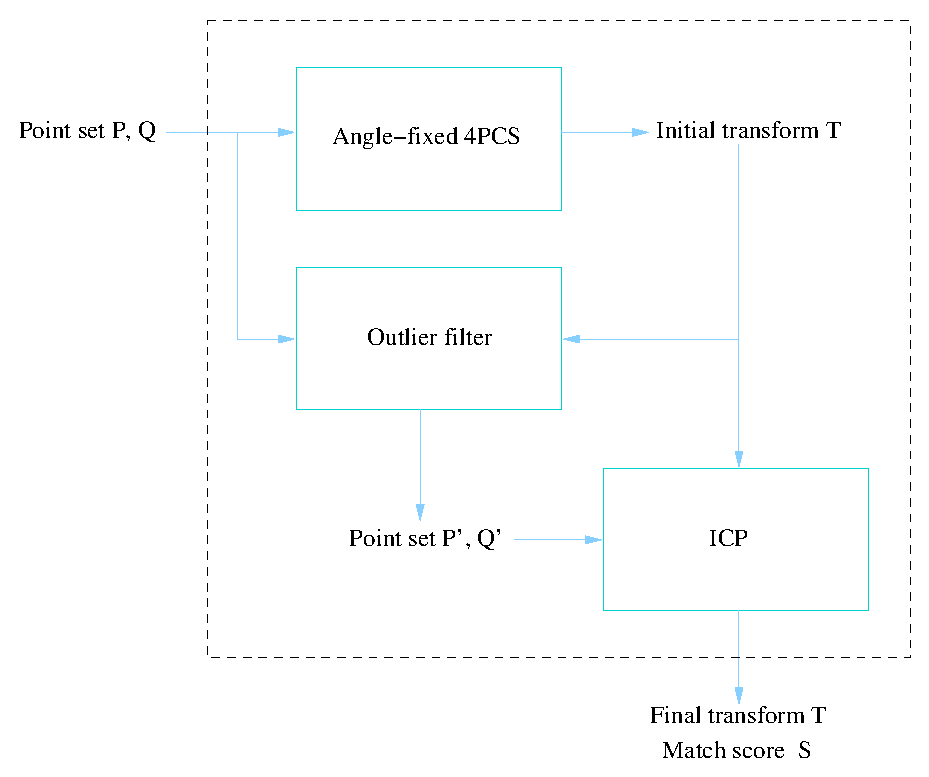
\includegraphics[width=12cm]{4pcs-pe}
  \caption{4PCS-PE算法框架}
  \label{fig:4pcs-pe}
\end{figure}
4PCS-PE由四个模块组成:Data preprocess、Modified 4PCS、Outlier filter和ICP,数据预处理模块根据输入的bbox或者mask在相机采集的深度图中获取对应的点集,并且将CAD模型通过采样转换为点集;Modified 4PCS是4PCS算法的优化版,也是4PCS-PE算法的核心,根据输入的两个点集,输出两个点集之间的粗略的变换关系;Outlier filter根据Modified 4PCS的输出对点集$P'$和$Q'$进行滤波,去掉一些离群点,用以提高下一步ICP算法的精度;ICP模块通过以Modified filter输出的变换关系为初始值对滤波后的两个点集进行迭代求解最佳的刚体变换关系,输出最终的变换关系$T$,也是目标的位姿。

\subsection{数据预处理}
数据预处理(Data preprocess)模块的核心任务有两个:
\begin{itemize}
\item 将CAD模型转换为点云
\item 从深度图中获取目标点云
\end{itemize}
对于将CAD模型转换为点云,基本思想是参考Uniform Sampling算法,Uniform Sampling算法的核心思想是以3D栅格中所有点的质心代替这些点,从而达到降采样。类似地,对于CAD模型也建立3D栅格,但由于无法获得3D栅格总所有点,因此判断CAD模型是否穿过3D栅格,如果穿过3D栅格,则在该3D栅格中心出增加一个点。显然3D栅格的边长越大,转换后的点云数量越小,精度越低,考虑到所使用相机生成点云的精度,因使CAD模型转换后的点云的精度与相机采集的点云的精度近似,实际取3D栅格边长为1mm,一个实际工件的CAD模型和以1mm为边长进行采样转换后的模型点云如图~\ref{fig:model-pc}~所示。
\begin{figure}[ht]
  \centering
  \subfloat[原CAD模型]{\includegraphics[width=7cm]{object-model}}
  \hskip1cm
  \subfloat[转换后点云]{\includegraphics[width=6cm]{object-pointcloud}}
  \label{fig:model-pc}
  \caption{CAD模型和转换后的点云}
\end{figure}

对于从深度图中获取目标点云则相对简单,只要将深度图中bbox或者mask所覆盖的像素通过深度摄像头的内参矩阵反投影到三维空间即可,详细见第~\ref{chap:rgbd}~章。

\subsection{4PCS算法及其优化}
介绍4PCS算法的优化之前,首先先详细介绍一下4PCS算法,4PCS算法是一个对3D点集全局匹配的算法,即使所给的两个3D点集有小的重叠,4PCS都能给出较好的结果,并且对噪声有一定的鲁棒性。这种方法对初始位姿没有任何要求,其核心是从3D点集中提取出所有与给定平面4-points近似全等的共面4-points,该算法时间复杂度为$O(n^2+k)$,其中$n$是3D点集中点的个数,$k$是提取出的4-points个数。4PCS使用十分广泛,并且引申出许多相关的变种\cite{corsini2013fully}。


\begin{algorithm}
  \caption{4PCS算法}
  \label{alg:4pcs}
  \KwIn{Point sets $P$ and $Q$, measure level $\delta$}
  \KwOut{Rigid transform $T$}
  $h\leftarrow 0$\;
  \For {$i = 1$ to $L$} {
    $B\leftarrow$ SELECTCOPLANARBASE($P$)\;
    $U\leftarrow$ FINDCONGRUENT($B,Q,\delta$)\;
    \ForAll {4-points coplannar sets $U_i\in U$} {
      $T_i\leftarrow$ best rigid transform that aligns $B$ to $U_i$ in the least square sense\;
      Find $S_i\subseteq P$, such that $d(T_i(S_i), Q)\leq\delta$\;
    }
    $k\leftarrow arg\;\underset{i}{max}\left\{|S_i|\right\}$\;
    \If {$|S_k| > h$} {
      $h\leftarrow |S_k|$\;
      $T\leftarrow T_k$\;
    }
    \Return $T$\;
  }
  \BlankLine
  \BlankLine
  \BlankLine
  \BlankLine
  \SetKwProg{Def}{def}{:}{}
  \Def{FINDCONGRUENT($B\equiv\left\{\mathbf{b_1},\mathbf{b_2},\mathbf{b_3},\mathbf{b_4}\right\},Q,\delta)$} {
    $d_1\leftarrow\;\parallel\mathbf{b_1}-\mathbf{b_2}\parallel$\;
    $d_2\leftarrow\;\parallel\mathbf{b_3}-\mathbf{b_4}\parallel$\;
    计算$R_1\equiv\left\{(\mathbf{p}_i,\mathbf{p}_j)\;|\;\mathbf{p}_i,\mathbf{p}_j\;\in Q\right\}$,使得$\parallel\mathbf{p}_i-\mathbf{p}_j\parallel\;\in [d_1-\delta,d_1+\delta]$\;
    计算$R_2\equiv\left\{(\mathbf{p}_i,\mathbf{p}_j)\;|\;\mathbf{p}_i,\mathbf{p}_j\;\in Q\right\}$,使得$\parallel\mathbf{p}_i-\mathbf{p}_j\parallel\;\in [d_2-\delta,d_2+\delta]$\;
    \ForAll {$r_{1i}\in R_1$} {
      计算与定量$r_1$和$r_2$相关的四个点$\left\{\mathbf{e}_{1i}^1,\mathbf{e}_{1i}^2,\mathbf{e}_{1i}^3,\mathbf{e}_{1i}^4\right\}$,记$\Pi(\mathbf{e}_{1i}^j)=r_{1i}$\;
    }
    对点集$\left\{\mathbf{e}_{1i}^j\right\}$在$\mathbb{R}^3$空间建立range tree(RS)\;
    \ForAll {$r_{2i}\in R_1$} {
      计算与定量$r_1$和$r_2$相关的四个点$\left\{\mathbf{e}_{2i}^1,\mathbf{e}_{2i}^2,\mathbf{e}_{2i}^3,\mathbf{e}_{2i}^4\right\}$,记$\Pi(\mathbf{e}_{1i}^j)=r_{1i}$\;
    }
    $U'\leftarrow\varnothing$\;
    \ForAll {$\mathbf{e}_{2i}^j$} {
      在RS中以$\delta$为领域检索点$\mathbf{e}_{2i}^j$附近的点,对于每个检索到的点$\mathbf{q}$,建立与$B$相对应的4个点的点集$U'\leftarrow\left\{U',(\Pi(\mathbf{q}),\Pi(\mathbf{e}_{2i}^j))\right\}$\;
    }
    \Return $U'$\;
  }
\end{algorithm}

\subsection{ICP算法}
ICP(Iterative Closest Point)算法,即最近点迭代算法,是最为经典的数据配准算法。ICP算法本质上是基于最小二乘法的最优配准方法。该算法重复进行选择对应关系点对,计算最优刚体变换,直到满足正确配准的收敛精度要求。由于ICP算法是一种迭代算法,因此只要时间允许便可以获取足够精度的解,但也正因为如此,ICP也容易陷入局部最优解。本文充分考虑了ICP算法的这个特点,通过Modified 4PCS算法给出初始的刚体变换来避免ICP算法陷入局部最优解,同时通过迭代来提高最后输出的刚体变换精度。下面介绍一下ICP算法的基本原理。

给定两个点集$P_n:=\left\{\mathbf{p}_1,\mathbf{p}_2,\ldots,\mathbf{p}_n\right\}$和$Q_m:=\left\{\mathbf{q}_1,\mathbf{q}_2,\ldots,\mathbf{q}_m\right\}$,以及初始旋转变换$R$和平移变换$t$,以及迭代结束额距离误差$\delta$,ICP算法迭代步骤如下:
\begin{itemize}
\item {\kai 步骤1:}根据当前$R$和$t$,对于点集$P_n$中的每个点在$Q_m$中找出距离最近的点,构成点集$Q_n$;
\item {\kai 步骤2:}计算$P_n$和$Q_n$之间的距离的均方根误差:
  \begin{equation}
    E(R,t) = \frac{1}{n}\sum_{i=1}^n{\parallel \mathbf{q}_i - R\mathbf{p}_i - t\parallel}
  \end{equation}
  通过奇异值分解求得使得$E(R,t)$最小的$R'$和$t'$;
\item {\kai 步骤3:}如果$E(R,t) < \delta$,结束迭代;否则$R\leftarrow R'$,$t\leftarrow t'$,跳转至步骤1。
\end{itemize}

ICP算法的迭代过程还是相对来说十分简单的,唯一需要思考一下的是如何求得最小化$E(R,t)$的$R'$和$t'$,通过奇异值分解求解$R'$和$t'$的方法如下:

首先,记
\begin{equation}
  \left\{
  \begin{array}{ccccc}
  P_n'& = &\left\{\mathbf{p}_i-\mathbf{\mu}_p \;|\; \forall \mathbf{p}_i \in P_n\right\}&:=&\left\{\mathbf{p}'_i\right\}\\
  Q_n'& = &\left\{\mathbf{q}_i-\mathbf{\mu}_q \;|\; \forall \mathbf{q}_i \in Q_n\right\}&:=&\left\{\mathbf{q}'_i\right\}
  \end{array}
  \right.
\end{equation}
其中
\begin{equation}
  \left\{
    \begin{array}{ccc}
      \mathbf{\mu}_p&=&\frac{1}{n}\sum_{i=1}^n{\mathbf{p}_i}\\
      \mathbf{\mu}_q&=&\frac{1}{n}\sum_{i=1}^n{\mathbf{q}_i}
    \end{array}
  \right.
\end{equation}
再另
\begin{equation}
  W = \sum_{i=1}^n{\mathbf{p}_i'\mathbf{q}_i'}
\end{equation}
然后对矩阵$W$进行奇异值分解:
\begin{equation}
  W = U\Sigma V^T
\end{equation}
则
\begin{equation}
  \left\{
    \begin{array}{ccc}
      R'&=&UV^T \\
        t'&=&\mathbf{\mu}_p-R'\mathbf{\mu}_q
    \end{array}
    \right.
\end{equation}



\section{位姿估计实验}


%%% Local Variables:
%%% TeX-master: "../thesis.tex"
%%% End: